\documentclass[paper=a4,fontsize=12pt,ngerman]{scrartcl}

\usepackage[utf8]{inputenc}				
\usepackage[T1]{fontenc}
\usepackage{graphicx}
\usepackage[ngerman]{babel}
\usepackage{amsmath}
\usepackage[a4paper,left=25mm,right=35mm,top=25mm,bottom=30mm]{geometry}
\usepackage{parskip}

\usepackage{tcolorbox}
\tcbuselibrary{listingsutf8}
\usepackage{listings}

\usepackage{verbatim} % in the preamble
\usepackage{subcaption}  % in your preamble
\usepackage{float}
	

\begin{document}

\pagenumbering{roman}
\pagestyle{plain}

% Einbinden der Titelseite
\begin{titlepage}

\linespread{1.5}


\includegraphics[width=\linewidth]{graphics/htw_logo}

\begin{center}
    \large  
    \hfill
    \vfill
    \Large{\bfseries{Netzwerkstaukontrolle und die Arbeitsweise verschiedener Algorithmen in TCP}}\\
    
    von \\
    Michał Roziel

    Matrikelnummer : 5012845

    \vfill
		
    Ein wissenschaftlicher Bericht im Rahmen der Vorlesung\\
    \glqq Wissenschaftliches Arbeiten\grqq\\
    an der htw saar im Studiengang Informatik\\
	
    \vfill	
    \vfill
	
    Saarbrücken, den 30. August 2025
\end{center}
    
\end{titlepage}


% Hier ist der Abstract
\section*{Abstract}



Dieser Bericht zielt darauf ab, aktuell benutzte Algorithmen der Netzwerkstaukontrolle in Computernetzwerken 
zu vergleichen.

Die Algorithmen der Staukontrolle, welche in diesen Vergleich einfließen sind : TCP BBR,
TCP NewReno, TCP Cubic, und TCP Vegas.  \newline

Mittels des Open-Source Netzwerksimulators \textit{NS-3} wird ein virtuelles Netzwerk mit einer 10Mbit/s Engstelle zwischen zwei Endpunkten aufgestellt. 
In diesem Netzwerk wird zunächst ein künstlicher Datenverkehr erzeugt.
Der genannte Datenverkehr wird anschließend aufgezeichnet und das dabei entstehende \textit{Congestion Window}(CW) dient als Basis für den Vergleich.
Die unterschiedlichen CW's werden schließlich analysiert und in Bezug auf das gegebene Szenario evaluiert.
Dieser Bericht bietet dem Leser einen Überblick über einige CC-Algorithmen und ein grundlegendes Verständnis darüber, wie Computernetzwerke auf Datenstau und 
Paketverlust reagieren.




\newpage
\section*{Selbstständigkeitserklärung}
Ich versichere, dass ich die vorliegende Arbeit selbstständig verfasst und 
keine anderen als die angegebenen Quellen und Hilfsmittel benutzt habe.
Insbesondere habe ich alle KI-basierten Werkzeuge angegeben, die ich bei
der Erstellung, Übersetzung oder Überarbeitung des Textes verwendet habe.

Ich erkläre hiermit weiterhin, dass die vorgelegte Arbeit zuvor weder von mir 
noch von einer anderen Person an dieser oder einer anderen Hochschule 
eingereicht wurde.

Darüber hinaus ist mir bekannt, dass die Unrichtigkeit dieser Erklärung eine 
Benotung der Arbeit mit der Note \glqq nicht ausreichend\grqq \ zur Folge hat 
und einen Ausschluss von der Erbringung weiterer Prüfungsleistungen zur Folge 
haben kann.
\bigskip
 
Saarbrücken, den \today

\smallskip
Unterschrift  Micha\l{} Roziel




% Das Inhaltsverzeichnis
\clearpage
\tableofcontents 

\clearpage
\pagenumbering{arabic}

% Hier beginnt das erste Kapitel


\section{Einleitung}

Network congestion control (CC) ist ein essentieller Bestandteil der 
meisten modernen Computernetzwerke. 
Wenn eine Netzwerkschnittstelle zu einem Zeitpunkt versucht eine zu große Menge an Datenpaketen aufzunehmen,
kommt es zu Stau von Datenverkehr und zu einem potentiellen Verlust von Datenpaketen.
Aufgrund diesem Vorkommen werden Algorithmen innerhalb von Netzwerkprotokollen verwendet, diese erkennen den Anstau von Datenverkehr im Netzwerk,
und helfen den Fluss von Datenpaketen zu steuern. Neben dem effizienten Durchfluss von Informationen ist zeitgleich auch die Fairness, 
was die Verteilung von Ressourcen einer Netzwerkschnittstelle an ihre Hosts angeht, wichtig. Auch dies wird von CC-Algorithmen gewährleistet.
In dem heutigen Stand von Rechnernetzen werden verschiedene Protokolle zur Netzwerkstaukontrolle verwendet, 
Ich werde mich im Rahmen dieses Berichts allerdings auf das Transmission Control Protocoll beschränken, da dies das am meisten verbreitete ist.  \newline
\newline
Mit stets weiterentwickelten Rechnernetzen, und einem jährlich zunehmenden Datenverkehr, wie auch in der Deutschen Internetschnittstelle
\textit{DE-CIX}\cite{DE-CIX2025} in Frankfurt gewinnen diese Algorithmen an Bedeutung. 






\subsection{Grundlagen und Begriffe}
Um die Funktionsweise und den Unterschied zwischen den hier behandelten CC-Algorithmen verstehen zu können, muss der Leser erst ein Grundverständnis über die Kommunukation innerhalb von Computernetzwerken haben.
Grundsätzlich wird heutzutage eins von zwei am verbreitesten Protokollen verwendet, entweder 
TCP oder UDP. 

\subsubsection{Transmission Control Protocoll}

Das Transmission Control Protocoll (TCP) ist ein weit verbreitetes Netzwerkprotokoll. 
TCP lässt sich in zu der Schicht 4 (Transportschicht) in dem OSI-Modell einordnen, hierbei liegt es zwichen der Vermittlungs- und Kommunikationsschicht.
\newline TCP wurde 1981 unter RFC 793 erstmals standarisiert. \cite{rfc793}  \newline
Die Aufgabes des TCP Protokolls ist es, zwischen zwei Hosts eine Verbindung aufzubauen, welche anschließend dazu genutzt wird,  
Nachrichten in zu verschicken und zu empfangen.

% QUOTE
\begin{quote}
``transport-layer protocol [\dots] from an application’s perspective, it is as if 
the hosts running the processes were directly connected;'' \cite[241]{kr22}.      
\end{quote}


Dies Bedeutet, dass TCP ebenfalls eine gewisses Abstraktionsniveau
des Nachrichtenaustausches abnimmt. 


Ein klares Unterscheidungsmerkmal des TCP von dem ebenfalls bekannten User Datagramm Protocoll (UDP) ist, dass TCP verbindungsorientiert arbeitet, 
während UDP als verbindungslos gilt. Zudem werden bei TCP Daten in Form von Packets verschickt, während man bei UDP von Datagrammen spricht. \newline
Bei TCP wird zu Beginn ein \textit{Three-Way-Handshake}
wie folgt durchgeführt : 

Der Sender schickt zunächst eine Nachricht mit einem Verbindungswunsch an den Empfänger und setzt das Flag 
\textit{Synchronize, \textbf{SYN}}.
\newline
Der Empfänger antwortet mit einer Bestätigung die erste Nachrichte erhalten zu haben, und schickt ebenfalls einen 
Verbindungswunsch. Es werden die Flags \textit{\textbf{SYN-ACK}} (Synchronise-Acknowledge) gesetzt.


Als letztes schickt der Sender eine Bestätigung, dass die Nachricht des Empfängers angekommen ist, dies geschieht wieder
mit dem Flag \textit{\textbf{ACK}}. Nun ist die Verbindung bereit, Daten in beide Richtungen zu übertragen.
Nach jedem gesendeten Datenpaket folgt eine \textit{\textbf{ACK}} Bestätigung.
\newline Die Abbildung \ref{fig:three-way-handshake} im Anhang visualisiert den Three-Way—Handshake.





\subsection{Algorithmen der Staukontrolle }

Algorithmen der Staukontrolle kommen zum Einsatz, wenn in einem Netzwerk ein potentieller Datenstau erkannt wird.
Grundsätzlich starten die Algorithmen in dem Arbeitsmodus \textit{slow start}.
Falls Datenstau erkannt wird, treten diese Algorithmen in die Phase \textit{congestion avoidance}.


 Hiermit wird mit verschiedenen Vorgehensweisen gegen die Netzwerküberlastung gesteuert. 
\newline
Es existieren unterschiedliche Typen von CC-Algorithmen, die jeweils ihre eigenen Vor- und Nachteile haben.
In diesem Bericht wird jeweils ein Algorithmus pro Typ behandelt.





\subsubsection{TCP BBR} 
Der \textit{Bottleneck Bandwith and Round-Trip-Time} Algorithmus wurde erstmals in dem von der
\textit{Association for Computing Machinery} (ACM) veröffentlichten Magazin ACM vorgestellt.\cite{cardwell2016bbr}. 

Seit 2016 wurden 3 Versionen entwickelt. Diese werden jeweils mit \textit{BBRv\_x} gekennzeichnet, 
wobei \textit{x} die entsprechende Version beschreibt. \newline
BBR ist ein modellbasiertes Staukontrollverfahren, dessen Arbeitsweise in 4 Phasen
unterteilt werden kann : \newline

\begin{enumerate}
    \item \textit{STARTUP}(Startphase)
    \item \textit{DRAIN}(Abbau des Staus)
    \item \textit{PROBE\_BW}(Proben der Bandweite)
    \item \textit{PROBE\_RTT}(Messen der Round-Trip-Time)
\end{enumerate}


Während andere CC-Algorithmen wie etwa Reno oder CUBIC auf Paketverlust reagieren, misst BBR die vorliegende Engpassbreite sowie RTT,
und bestimmt daraus die Sende-Rate, welche anschließend in dem Netzwerk eingesetzt wird. 
Da BBR nicht direkt auf Paketverlust reagiert, kommt es mit gut mit zufälligen Paketverlust zurecht, hat aber zeitgleich
Schwierigkeiten mit der Fairness was die Verteilung von Ressourcen angeht : 

% QUOTE

\begin{quote}
``Unfairness happens [\dots], which relates to different settings of round-trip times and buffer sizes.
Essentially, the reason for the unstable or unequal unfairness is the absence of responding mechanisms for bandwidth convergence.''\cite{tang24BBRns3}
\end{quote}
 

Die Fairness kann hierbei mit dem zwischen 0 und 1 liegenden Jain's Fairness Index gemessen werden.\cite{DBLP:journals/corr/cs-NI-9809099}

\subsubsection{TCP Reno}

\subsubsection{TCP Cubic}
Der Algorithmus TCP Cubic ist ein Loss-Based CC-Algorithmus, das bedeutet der
Arbeitsmodus \textit{congestion avoidance} tritt ein, falls ein Paketverlust erkannt wird.

Die Wachstumsfunktion, welche anschließend die neue Größe des \textit{Congestion Window}
beschreibt, wird definiert als : $ W(t) = C(t-K)^3 + W\text{max}.$  
Hierbei ist \textit{W} die größe des Congestion Windows, \textit{C} eine Cubic-Konstante, 
\textit{t} die Zeit seit dem letzten Paketverlust, \textit{K} die Zeit, welche \textit{TCP Cubic} benötigt 
um wieder \textit{W\text{max}} zu erreichen.

Mit der Sensitivität auf Paketverlust $\beta$ kann \textit{K} wie folgt berechnet werden :
\[
K = \sqrt[3]{\frac{W_{\text{max}} \cdot \beta}{C}}
\]



\subsubsection{TCP Vegas}

\clearpage

\subsubsection{Merkmale der CC Algorithmen auf einen Blick}

\begin{table}[ht]
\centering

\begin{tabular}{r|l|l|l}
   & \textbf{Algorithmus} & \textbf{Typ} & \textbf{Signal der Congestion avoidance} \\ \hline
\textbf{BBR} & a & b & c \\
\textbf{NewReno} & d & e & f \\
\textbf{Cubic} & g & h & i \\
\textbf{Vegas} & n & f & f 

\end{tabular}
\end{table}

\subsection{Definitionen}

\subsubsection{Queuing Delay}
Queuing Delay beschreibt das Warten einer \textit{Queue}
auf das Versenden von Packets durch das gegebene Netzwerk.

\clearpage
\section{Versuchsaufbau}

Mit einem Test innerhalb des Command Line Simulators \textit{NS-3.45} lässt sich ein beliebieger CC-Algorithmus ausführen.


\textbf{Netzwerktopologie}

Zunächst definieren wir die Netzwerktopologie auf welcher die CC-Algorithmen
laufen werden.\cite{ns3BBR}
\small
\begin{verbatim}
            1000 Mbps           10 Mbps           1000 Mbps
  Sender -------------- R1 -------------- R2 -------------- Receiver
             5 ms                10 ms              5 ms
\end{verbatim}
So ist es möglich, einen Netzwerkstau zu simulieren, dieser bleibt für jeden Algorithmus gleich.

Durch das Verändern der folgenden \textit{C++} Codezeile der Datei \textit{tcp-bbr-example.cc} mit dem Namen des gewünschten Algorithmus lässt sich der Test unter gleichen Netzwerkbedingungen für die anderen Tesstfälle ausführen :

\small
\begin{verbatim}
[...]
    std::string tcpTypeId = "ALGO_NAME";     
[...]
\end{verbatim}
Mittels der Navigation in das Directory \textit{ns-3.45} per Kommandozeile und dem Befehl
\small
\begin{verbatim}
    ./ns3 run examples/tcp/tcp-bbr-example.cc
\end{verbatim}
lässt sich der jeweilige Testlauf ausführen.
 Die aufgezeichneten Informationen können mit dem im Anhang 
 in \ref{sec:gnuplot-skript} hinterlegten Skript visualisiert werden.


\begin{figure}[H]
    \centering

    \begin{subfigure}{0.40\textwidth}

        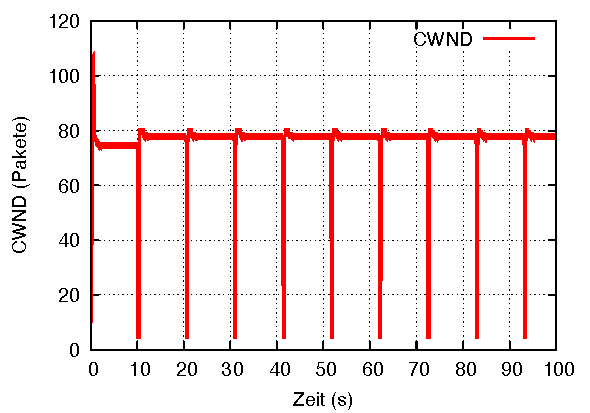
\includegraphics[width=\linewidth]{graphics/bbrCW.pdf}
        \caption{BBR}
        \label{fig:bbr}
    \end{subfigure}
    \hfill
    \begin{subfigure}{0.40\textwidth}
        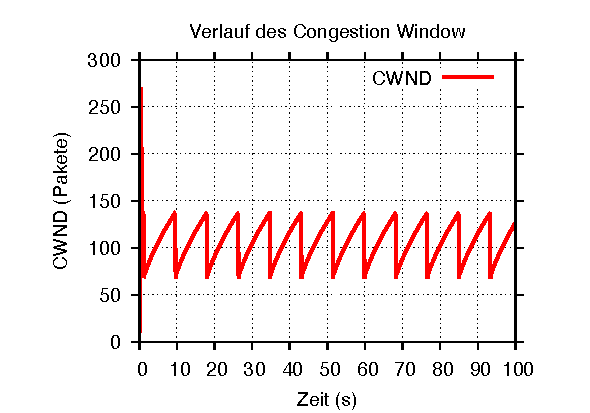
\includegraphics[width=\linewidth]{graphics/newRenoCW.pdf}
        \caption{NewReno}
        \label{fig:newreno}
    \end{subfigure}
    \hfill
    \begin{subfigure}{0.40\textwidth}
        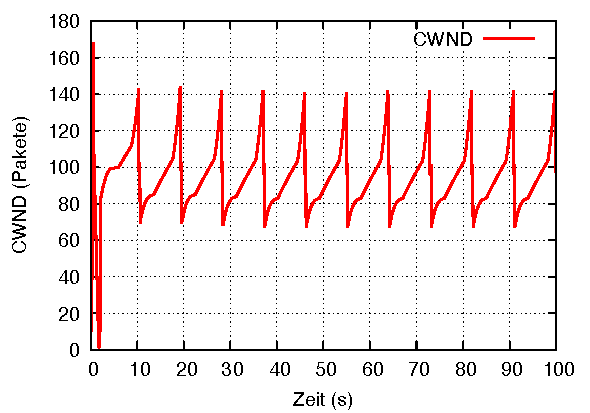
\includegraphics[width=\linewidth]{graphics/cubicCW.pdf}
        \caption{Cubic}
        \label{fig:cubic}
    \end{subfigure}
    \hfill
    \begin{subfigure}{0.40\textwidth}
        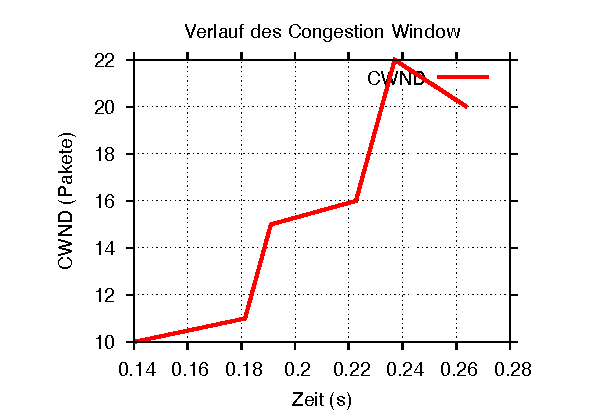
\includegraphics[width=\linewidth]{graphics/vegasCW.pdf}
        \caption{Vegas}
        \label{fig:vegas}
    \end{subfigure}

    \caption{Vergleich der aufgezeichneten Congestion Windows.}
    \label{fig:cwnd-all}
\end{figure}

\clearpage 
\subsection{Analyse der Ergebnisse}
Wie an den \textit{Congestion Window} Graphen erkennbar, besitzt jeder 
der vorgestellten Algorithmen eine eigene Herangehensweise was  das Regulieren 
von Datenstau angeht.


\section{Ergebnisse und Diskussion}


\section{Fazit und Schlussfolgerungen}


\subsection{Offene Fragen}


\subsection{Diskussion}


% Hier beginnt das Literaturverzeichnis
\clearpage
\renewcommand\refname{Literaturverzeichnis}
\bibliographystyle{ieeetr}
\bibliography{literatur}
\addcontentsline{toc}{section}{Literaturverzeichnis}


% Hier beginnt der Anhang
\clearpage
\appendix
\part*{Anhang}

\addcontentsline{toc}{section}{Anhang}

\subsection{Zusätzliche Abbildungen}

\begin{figure}[ht]
    \centering
    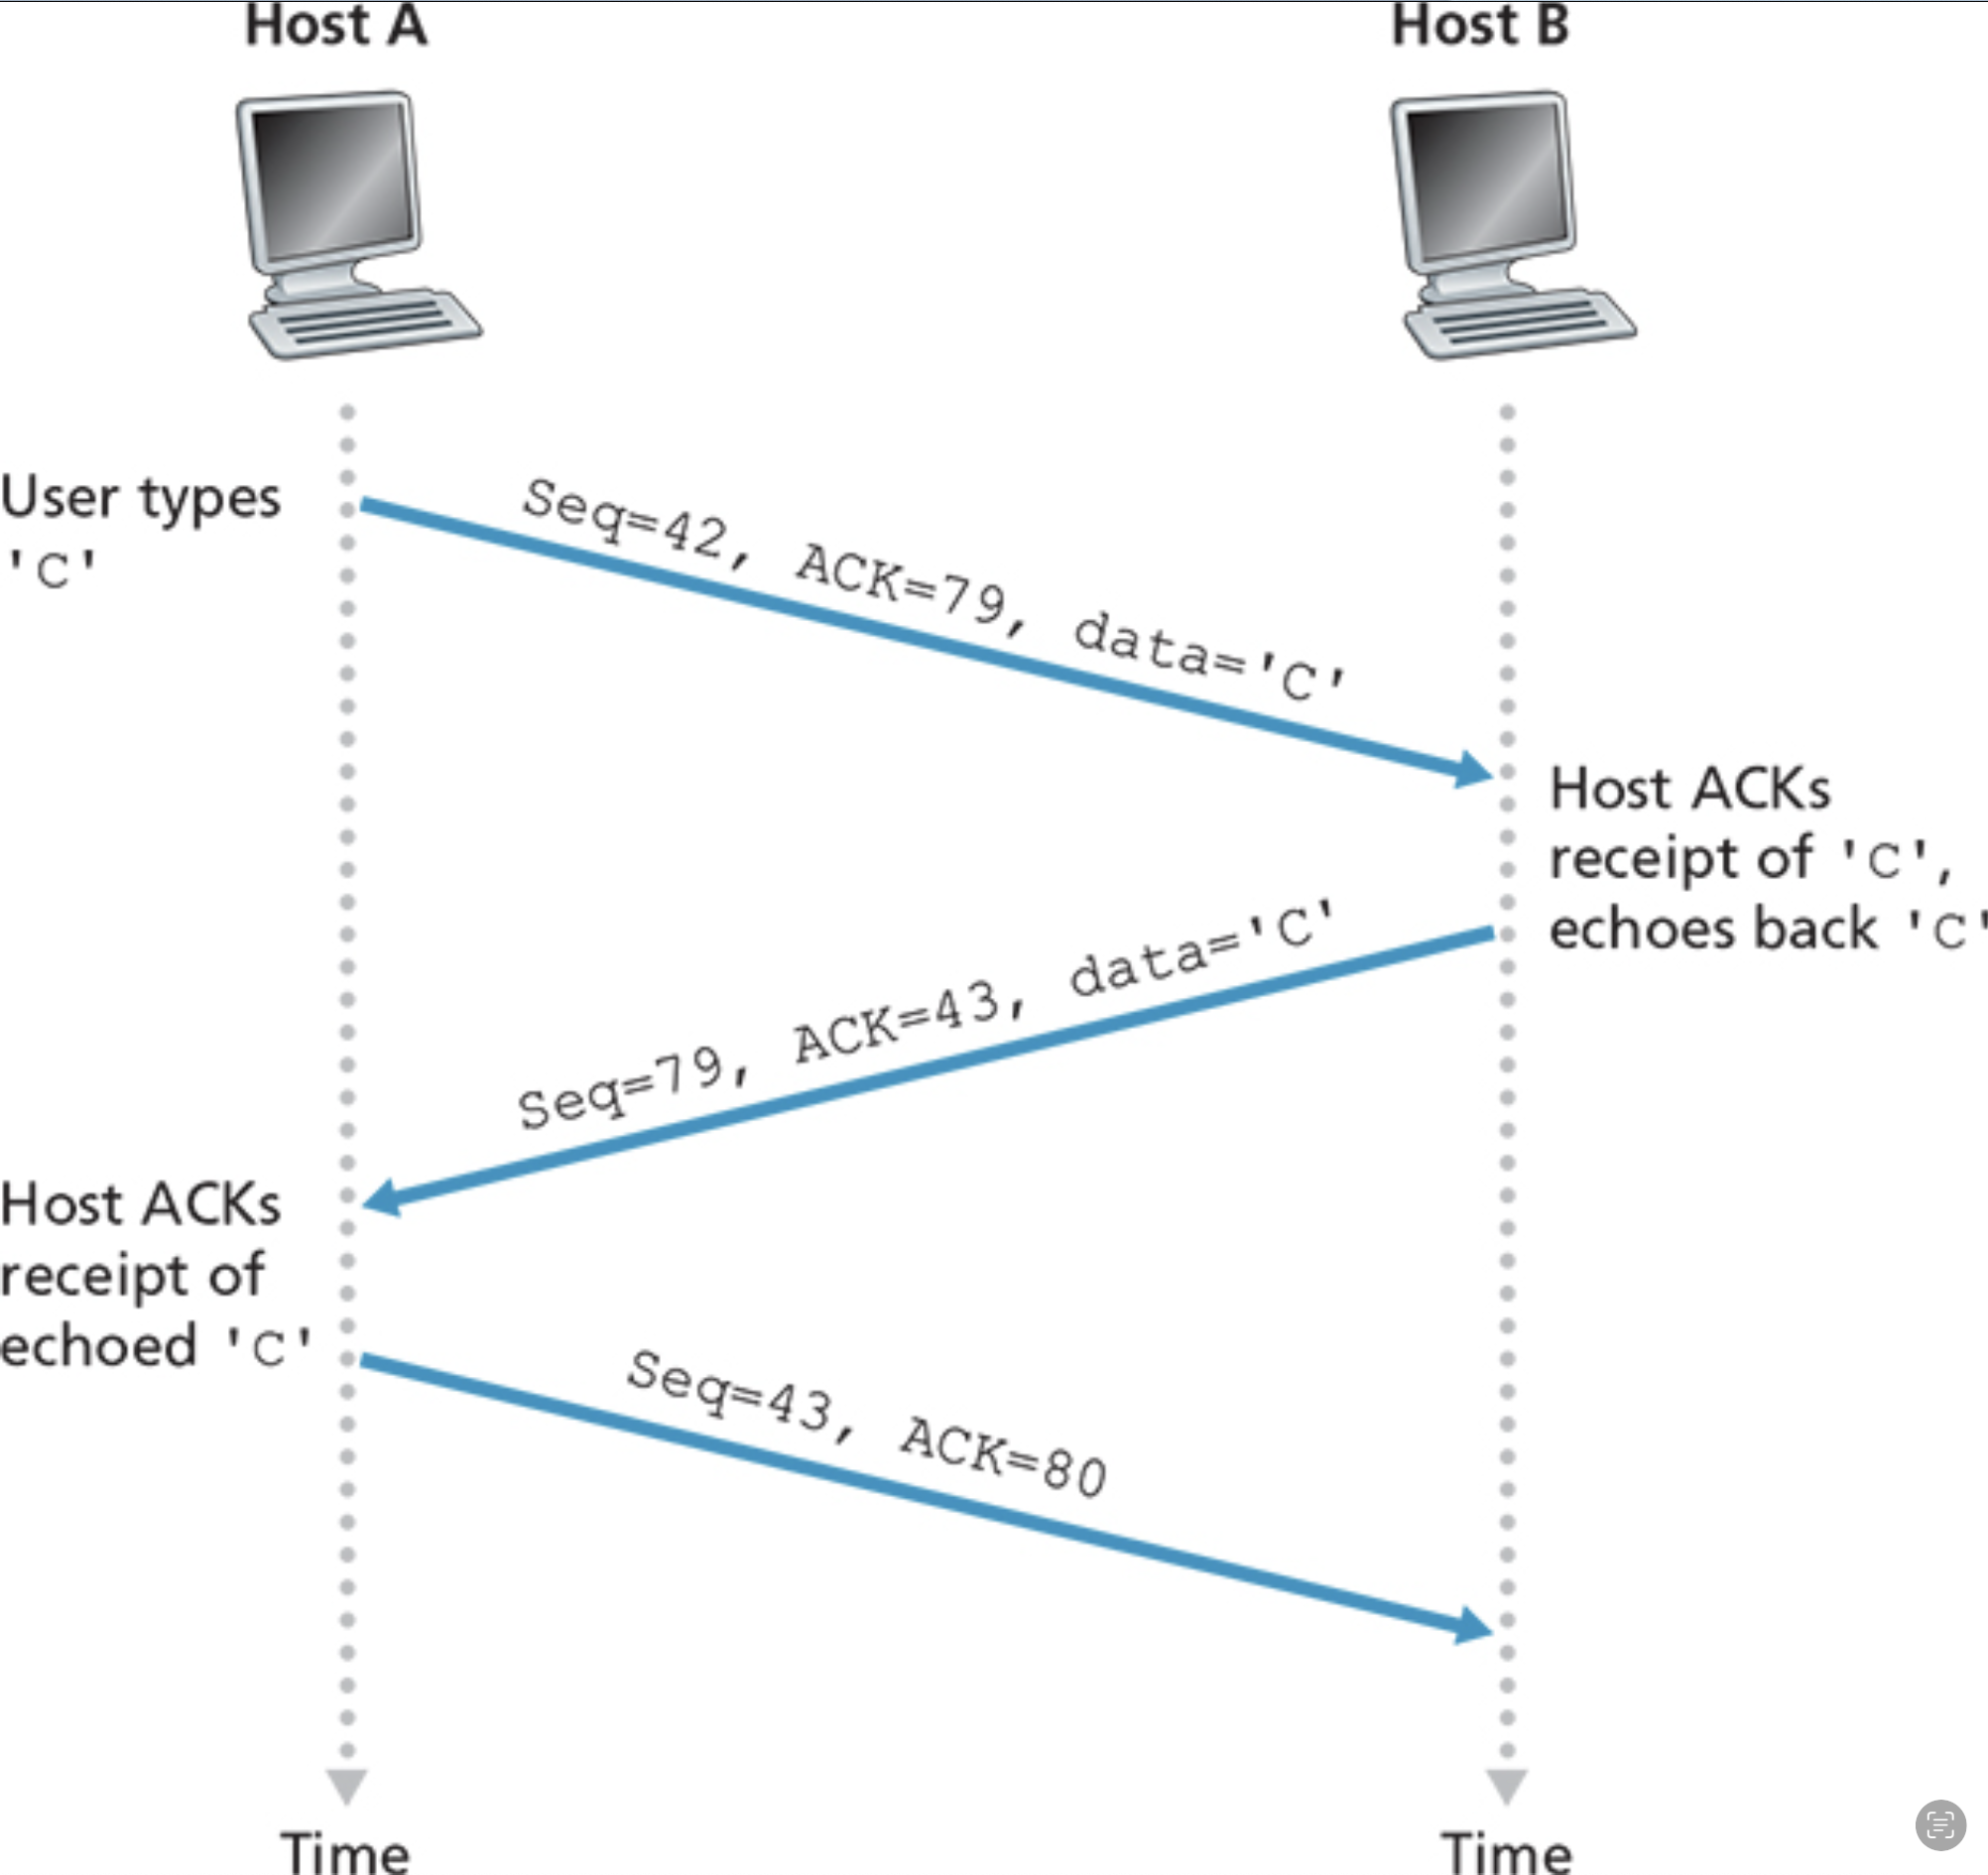
\includegraphics[height=10cm]{graphics/3way.png}
    \caption{Detaillierte Darstellung des Three-Way Handshake.}
    \label{fig:three-way-handshake}
\end{figure}



\subsection{GnuPlot Skript zur Erstellung der CWND Graphen}
\label{sec:gnuplot-skript}

\begin{verbatim}

set terminal pdfcairo size 10cm,7cm enhanced font "Helvetica,14"
set output "cwnd.pdf"

set xlabel "Zeit (s)"
set ylabel "CWND (Pakete)"
set grid
set key top right

plot "cwnd.dat" using 1:2 with lines lw 2 lc rgb "red" title "CWND"

\end{verbatim}


\section{Datenmaterial}


\section{Web-Standards}
O

\end{document}

